%
% Modellbildung
%
% @version 1.0
% @author dmayer
% @created 29. Dezember 2015

\setchapterpreamble[o]{%
\dictum[--- \textsc{Norbert Wiener}]{\Gun Das beste Modell für eine Katze ist eine Katze; möglichst dieselbe Katze. \Gob}}
\renewcommand{\chapterheadstartvskip}{\vspace*{2cm}}

\chapter{Modellbildung des Raumes}
\label{chap:modellbildung}

Ziel dieses Kapitels ist es, ein hinreichend exaktes Modell zur Berechnung der Raumtemperatur in K004b zu bilden. Die Modellbildung soll physikalisch motiviert sein und daher auf den thermodynamischen Prozessen mit der Außenumgebung und der Anlage aus Kapitel \ref{chap:anlagendesign} basieren. Des Weiteren soll das Modell speziellen Anforderungen genügen, um eine Modellprädiktive Regelung der Anlage zu ermöglichen.

Dazu wird zunächst ein einfaches Grundmodell für einen hypothetischen Raum gebildet, dass anschließend schrittweise an den bestehenden Raum erweitert angepasst wird, bis eine die Qualität/Güte des Modells ausreichend ist.

\section{Anforderungen an das Raummodell}
Die triviale Aufgabe des Modells ist eine hinreichend genaue Beschreibung der realen Vorgänge und des Temperaturverlaufs. Hinreichend bedeutet, dass das Modell eine ausreichende Güte für den Einsatz mit Modellprädiktiver Regelung besitzt. In Kapitel \ref{sec:mpc} wurden bereits die Grundlagen zur Modellprädiktiven Regelung erläutert, wodurch sich Einschränkungen bei der Modellbildung ergeben. Dabei wurde festgestellt, dass die Lösung von Optimalsteuerungsproblemen gradientenbasiert erfolgt und die zweifache Erzeugung von Ableitung erfordert. Damit ergibt sich die Anforderung, dass das Modell keine Unstetigkeiten aufweist und sich zweimal stetig differenzieren lässt.
Zudem ist Berechnung von Lösungen für Optimalsteuerungsprobleme sehr rechenintensiv und muss während des laufenden Betriebs der Anlage wiederholt stattfinden. Da die Lösung zudem wiederholt stattfinden muss
, wird eine erhöhte Rechenkapazität benötigt, 
um die Lösung in ausreichender Zeit zu berechnen. 

Daraus ergibt sich eine weitere Anforderung, denn um den Rechenbedarf möglichst gering zu halten, soll das Modell möglichst wenig KOmplexität besitzen.
Wie bereits bei den Anforderungen an die Anlage in Abschnitt \ref{sec:anforderungen} festgestellt wurde, stellt die Umgebung zur Optimalsteuerung einen begrenzenden Faktor dar, wodurch das Modell mit der Modellierungssprache Modelica gebildet wird.

Da diese Anforderungen teils gegenläufig sind, gilt es einen Kompromiss zu finden, ein stetig differenzierbares Modell,
, um eine ausreichende Modellgüte zu erhalten, gleichzeitig jedoch keine hohe Komplexität oder einen großen Umfang an Gleichungen besitzt.
Ziel: Hohe Modellgüte bei gleichzeitig geringer Komplexität und Stetigkeit

Daher wird im Folgenden zunächst ein simples Raummodell gebildet, dass anschließend sukzessive erweitert und damit die Komplexität des Modells schrittweise erhöht wird, bis eine ausreichende Beschreibung der Realität mit dem Modell möglich ist.

\section{Das Grundmodell des Raumes}

Um ein möglichst einfaches Grundmodell zu erhalten, wird zunächst ein hypothetischer Raum betrachtet. Dieser Raum bildet zusammen mit der ihn umgebenden Luft ein abgeschlossenes thermodynamisches System, wie in Kapitel \ref{sec:grundlagenmodell} beschrieben. Der Raum ist selbst mit Luft gefüllt und wird zu allen sechs Seiten hin durch Wände begrenzt. Damit bildet der Raum ein geschlossenes System, da keine Massenströme über die Grenzen hinweg fließen können. An den Grenzflächen kann also lediglich Wärme zwischen der Umgebung und dem  Raum ausgetauscht werden. Des Weiteren wird eine homogene Temperatur innerhalb des Raumes und der Umgebung angenommen, welche in der Realität eingeschwungenen Gleichgewichtszuständen innerhalb der beiden Teilsysteme entspricht. Um die Annahme für den Raum zu überprüfen, muss noch festgestellt werden auf welcher zeitlichen Skala der Einschwingvorgang für eine homogene Temperatur innerhalb des Raumes stattfindet und ob dieser damit eine Relevanz für die Modellbildung besitzt.

\begin{figure}
\centering
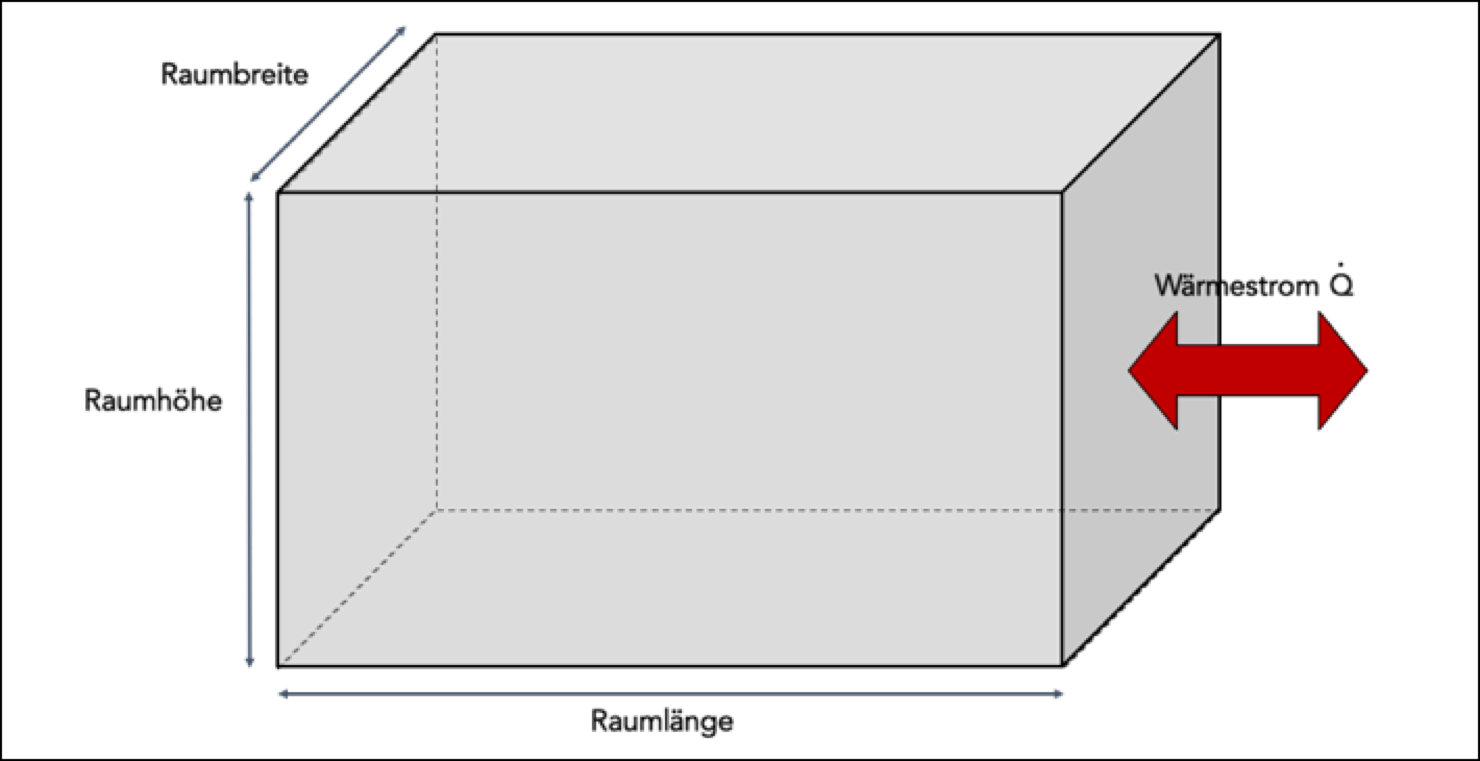
\includegraphics[width=\textwidth]{abbildungen/20160316_grundraum}
\caption{Grundmodell eines Raumes}
\label{fig:grundraum}
\end{figure}

Zur Bestimmung der Temperatur innerhalb des Raumes, ausgehend von einer initialen Raumtemperatur und dem externen Steuerungsparameter der Umgebungstemperatur, muss der Ausgleichsprozess zwischen Raum und Umgebung untersucht werden, konkret der ausgetauschte Wärmestrom. Um diesen nach \ref{eq:qdot} zu berechnen, müssen zunächst die verschiedene modellrelevanten Eigenschaften des Raumes durch physikalische Größen und Variablen beschrieben werden. Zur Berechnung der Austauschoberfläche wird die Raumbreite, -länge und -höhe benötigt und weiterhin sind der U-Wert einer Betonwand, die spezifische Wärmekapazität und Dichte von Luft für die Bestimmung des Wärmestroms relevant.
Diese modellrelevanten Eigenschaften sind allesamt mit ihren Zahlenwerten in Tabelle \ref{tab:eigenschaften_raum} zusammengefasst.

\begin{table}[H]
\centering
\small
\renewcommand{\arraystretch}{1.3}
\begin{threeparttable}
\begin{tabularx}{1\textwidth}{p{0.5\textwidth}m{0.2\textwidth}m{0.18\textwidth}}
\toprule
\textbf{Modellrelevante Eigenschaften} & \textbf{Wert} & \textbf{Einheit} \\
\cmidrule[0.5pt](r{0.25em}){1-1} 
\cmidrule[0.5pt](l{0.25em}){2-2}
\cmidrule[0.5pt](l{0.25em}){3-3}

Raumbreite & 7,81\tnote{1)} & $[m]$ \\ 
\ccol Raumlänge & \ccol 5,78\tnote{1)} & \ccol $[m]$ \\
Raumhöhe & 2,99\tnote{1)} & $[m]$ \\
\ccol Wärmedurchgangskoeffizient Betonwand & \ccol 2,0\tnote{2)} & \ccol $[\frac{W}{m^{2}*K}]$\\
Spezifische Wärmekapazität von Luft & 1.000,0\tnote{3)} & $[\frac{J}{kg*K}]$\\
\ccol Dichte von Luft & \ccol 1,25 \tnote{3)} & \ccol $[\frac{kg}{m^{3}}]$\\
\bottomrule
\end{tabularx}
\begin{tablenotes}[]\footnotesize\singlespacing\setlength\labelsep{0pt}
\item[1)] Werte durch eigene Vermessung des Raumes K004b vom 07.12.2015.
\item[2)] Schätzwert, geschätzt nach \cite[S.~409]{re14} mit Richtwerten aus \cite[S.~194ff.]{re14}.
\item[3)] Tabellenwert aus \cite[S.~139]{ha13}.
\end{tablenotes}
\end{threeparttable}
\caption{Eigenschaften des Raummodells}
\label{tab:eigenschaften_raum}
\end{table}

Erfolgt nun die Bilanzierung des Raumes mit Hilfe des ersten Hauptsatzes der Thermodynamik nach \ref{eq:hauptsatz} und die Berechnung der inneren Energie des Raumes nach \ref{eq:innereenergie} ergibt sich folgendes, einfaches Gleichungssystem zur Bestimmung der Raumtemperatur in Abhängigkeit vom Steuergrößen Außentemperatur im Grundmodell in Modelica:

\begin{lstlisting}[language=Modelica,caption={Einfaches Gleichungssystem für das Grundmodell des Raumes in Modelica}, label=lst:grundraum]
equation
   /* calculate room volume */
   room_volume = room_length * room_height * room_breadth;
   /* calculate room mass */
   room_mass = room_volume * rho_air;
   /* calculate surface of heat exchange */
   exchange_surface = 2 * (room_length * room_breadth) + 2 * (room_length * room_height) + 2 * (room_breadth * room_height);
   /* calculate inner energy*/
   room_u = room_mass * cp_air * room_temperature;
   /* calculate derivative of the inner energy */
   der(room_u) = environment_qdot;
   /* calculate heatflow between room and environment */
   environment_qdot = u_wall * exchange_surface * (environment_temperature - room_temperature);
\end{lstlisting}

Damit ist ein Grundmodell für einen Raum gebildet, wie in \ref{fig:grundraum} graphisch dargestellt, um die Temperatur innerhalb eines Raumes zu berechnen. Dieses wird im Folgenden nun schrittweise erweitert und zum Abschluss überprüft, ob es der Realität genüge zu trägt.


\section{Modellerweiterung durch Berücksichtigung der realen Umgebung}

Im nächsten Schritt wird das einfache Raummodell zunächst an die reale Umgebung des Raums K004b angepasst. Die Lage von K00b ist in \ref{fig:skizzek004a} ersichtlich und es ist zu erkennen, dass der Raum lediglich zwei Außenwände besitzt, die an die Umgebungsluft grenzen: Die Wände in Richtung Süden und Westen. Die anderen beiden Wände, sowie die Decke und der Boden, grenzen an weitere Gebäudeteile des K~Gebäudes. Somit entspricht der Raum im Modell nach wie vor einem geschlossenen System und bildet weiterhin, zusammen mit dem umgebenden K~Gebäude und der Umgebungsluft, ein abgeschlossenes System. Jedoch müssen nun potenziell verschiedene Wärmeströme zwischen dem Raum und der Außenumgebung sowie dem Raum und dem K~Gebäude betrachtet werden. Da die fließenden Wärmeströme im Vergleich zur sehr großen Energie innerhalb des gesamten K~Gebäudes und der Umgebung nur verschwindend gering sind, wird der erwärmende beziehungsweise kühlende Effekt der Wärmeströme auf die beiden Teilsysteme vernachlässigt und es wird von konstanten, homogenen Temperaturen beider ausgegangen.

Durch diese Erweiterung des Modells hängt die Raumtemperatur nun von zwei Wärmeströmen und damit indirekt von zwei externen Steuergrößen, den Temperaturen in der Umgebung und im K~Gebäude, ab. Um die Wärmeströme separat berechnen zu können, wird die gesamte Oberfläche zum Wärmeaustausch aufgeteilt in die Austauschoberfläche mit der Umgebung und die Austauschoberfläche mit dem K~K~GebäudeGebäude. Des Weiteren werden im Modell die Temperatur der Außenumgebung und die Temperatur innerhalb des K~Gebäudes als externe Steuergrößen berücksichtigt. Das Gleichungssystem des Grundmodells in \ref{lst:grundraum} erweitert sich also um folgende Änderungen:

\begin{lstlisting}[language=Modelica, caption={Erweitertes Gleichungssystem Modell des Raumes unter Berücksichtigung der realen Umgebung in Modelica}, label=lst:raumeins]
equation
   [...]
   /* calculate surface of heat exchange with the environment */
   environment_surface = room_length * room_height + room_breadth * room_height;
   /* calculate surface of heat exchange with the remaining building */
   building_surface = 2 * (room_length * room_breadth) + room_length * room_height + room_breadth * room_height;
   /* calculate derivative of the inner energy */
   der(room_u) = environment_qdot + building_qdot;
   /* calculate heatflow between room and environment */
   environment_qdot = u_wall * environment_surface * (environment_temperature - room_temperature);
   /* calculate heatflow between room and building */
   building_qdot = u_wall * building_surface * (building_temperature - room_temperature);
\end{lstlisting}

Damit wurde das Raummodell an die reale Umgebung angepasst und um die Temperatur innerhalb des Raumes zu bestimmen, wird nun neben der Ausgangstemperatur im Raum und der Umgebungstemperatur noch die Temperatur innerhalb des restlichen K~Gebäudes berücksichtigt. Im nächsten Schritt werden die realen, räumlichen Gegebenheiten im Modell abgebildet.


\section{Modellerweiterung durch Berücksichtigung der räumlichen Gegebenheiten}

Um das Modell an die realen Gegebenheiten des Raumes K004b anzupassen, müssen zwei bauliche Gegebenheiten beachtet werden. Wie in \ref{fig:skizzek004a} bereits dargestellt ist, ist in der südlichen Außenwand eine Fensterfront vorhanden. Da der U-Wert eines Fensters erheblich von dem U-Wert einer Wand abweicht, entsteht ein zusätzlicher Wärmestrom zwischen dem Raum und der Umgebung durch das Fenster hindurch. Das Öffnen und Schließen der Fenster mit daraus resultieren Massenströmen wird zunächst nicht explizit berücksichtigt, weshalb das Raummodell weiterhin als geschlossenes System betrachtet wird. Des Weiteren ist es möglich, den Raum über einen Heizkörper zu beheizen. Mit dem Heizkörper, der zunächst als einfache Wärmequelle im Modell ergänzt wird, erhöht sich die Anzahl der externen Steuergrößen erneut, da die Temperatur innerhalb des Raumes auch von dieser abhängig ist.

Durch diese Erweiterungen werden auch weitere physikalische Größen zur Beschreibung der Eigenschaften des Raummodells benötigt. Wie bereits erwähnt werden die Eigenschaften um den U-Wert eines Fensters, sowie die Breite und Höhe der Fensterfront ergänzt, wie in Tabelle \ref{tab:eigenschaften_raumerw} zusammengefasst.

\begin{table}[H]
\centering
\small
\renewcommand{\arraystretch}{1.3}
\begin{threeparttable}
\begin{tabularx}{1\textwidth}{p{0.5\textwidth}m{0.2\textwidth}m{0.18\textwidth}}
\toprule
\textbf{Modellrelevante Eigenschaften} & \textbf{Wert} & \textbf{Einheit} \\
\cmidrule[0.5pt](r{0.25em}){1-1} 
\cmidrule[0.5pt](l{0.25em}){2-2}
\cmidrule[0.5pt](l{0.25em}){3-3}

Fensterbreite & 7,0\tnote{1)} & $[m]$ \\ 
\ccol Fensterhöhe & \ccol 2,08\tnote{1)} & \ccol $[m]$ \\
Wärmedurchgangskoeffizient Glas & 4,0\tnote{2)} & $[\frac{W}{m^{2}*K}]$\\

\bottomrule
\end{tabularx}
\begin{tablenotes}[]\footnotesize\singlespacing\setlength\labelsep{0pt}
\item[1)] Werte durch eigene Vermessung des Raumes K004b vom 07.12.2015.
\item[2)] Tabellenwert, geschätzt nach \cite[S.~270ff.]{h2000}.
\end{tablenotes}
\end{threeparttable}
\caption{Weitere Eigenschaften des Raummodells}
\label{tab:eigenschaften_raumerw}
\end{table}
 
Durch diese Anpassung verändert sich die Austauschoberfläche mit der Umgebung, die sich nun auf zwei Flächen mit verschiedenen Wärmedurchgangskoeffizienten verteilt. Des Weiteren wird eine Wärmequelle für die Heizung ergänzt, so dass sich folgende Änderungen des Gleichungssystems im Vergleich zum bisherigen Modell in \ref{lst:grundraum} ergeben:

\begin{lstlisting}[language=Modelica, caption={Erweitertes Gleichungssystem des Raumes unter Berücksichtigung der räumlichen Gegebenheiten in Modelica},label=lst:raumzwei]
equation
   [...]
   /* calculate surface of heat exchange with the environment */
   environment_surface = room_length * room_height + room_breadth * room_height - window-surface;
   /* calculate surface of heat exchange with the remaining building */
   building_surface = 2 * (room_length * room_breadth) + room_length * room_height + room_breadth * room_height;
   /* calculate surface of window with the environment */
   window_surface=(window_length*window_height);
   /* calculate derivative of the inner energy */
   der(room_u) = environment_qdot + building_qdot + window_qdot + radiator_qdot;
   /* calculate heatflow between room and environment through the walls */
   environment_qdot = u_wall * environment_surface * (environment_temperature - room_temperature);
   /* calculate heatflow between room and environment through the window */
   building_qdot = u_glass * window_surface * (environment_temperature - room_temperature);
   /* calculate heatflow between room and building */
   building_qdot = u_wall * building_surface * (building_temperature - room_temperature);
\end{lstlisting}

Damit ist das Modell auch an die räumlichen Gegebenheiten angepasst und beschreibt dadurch die realen Zusammenhänge in groben Zügen. Die bisherigen Zusammenhänge des Modells sind in \ref{fig:raumeins} graphisch dargestellt. Allerdings kann ein Controller die Heizung nicht beliebig als einfache Wärmequelle einsetzen. Daher wird im folgenden Abschnitt ein detaillierteres Modell des Heizkörpers gebildet, um die Steuerung für den Controller zu ermöglichen. 

\begin{figure}
\centering
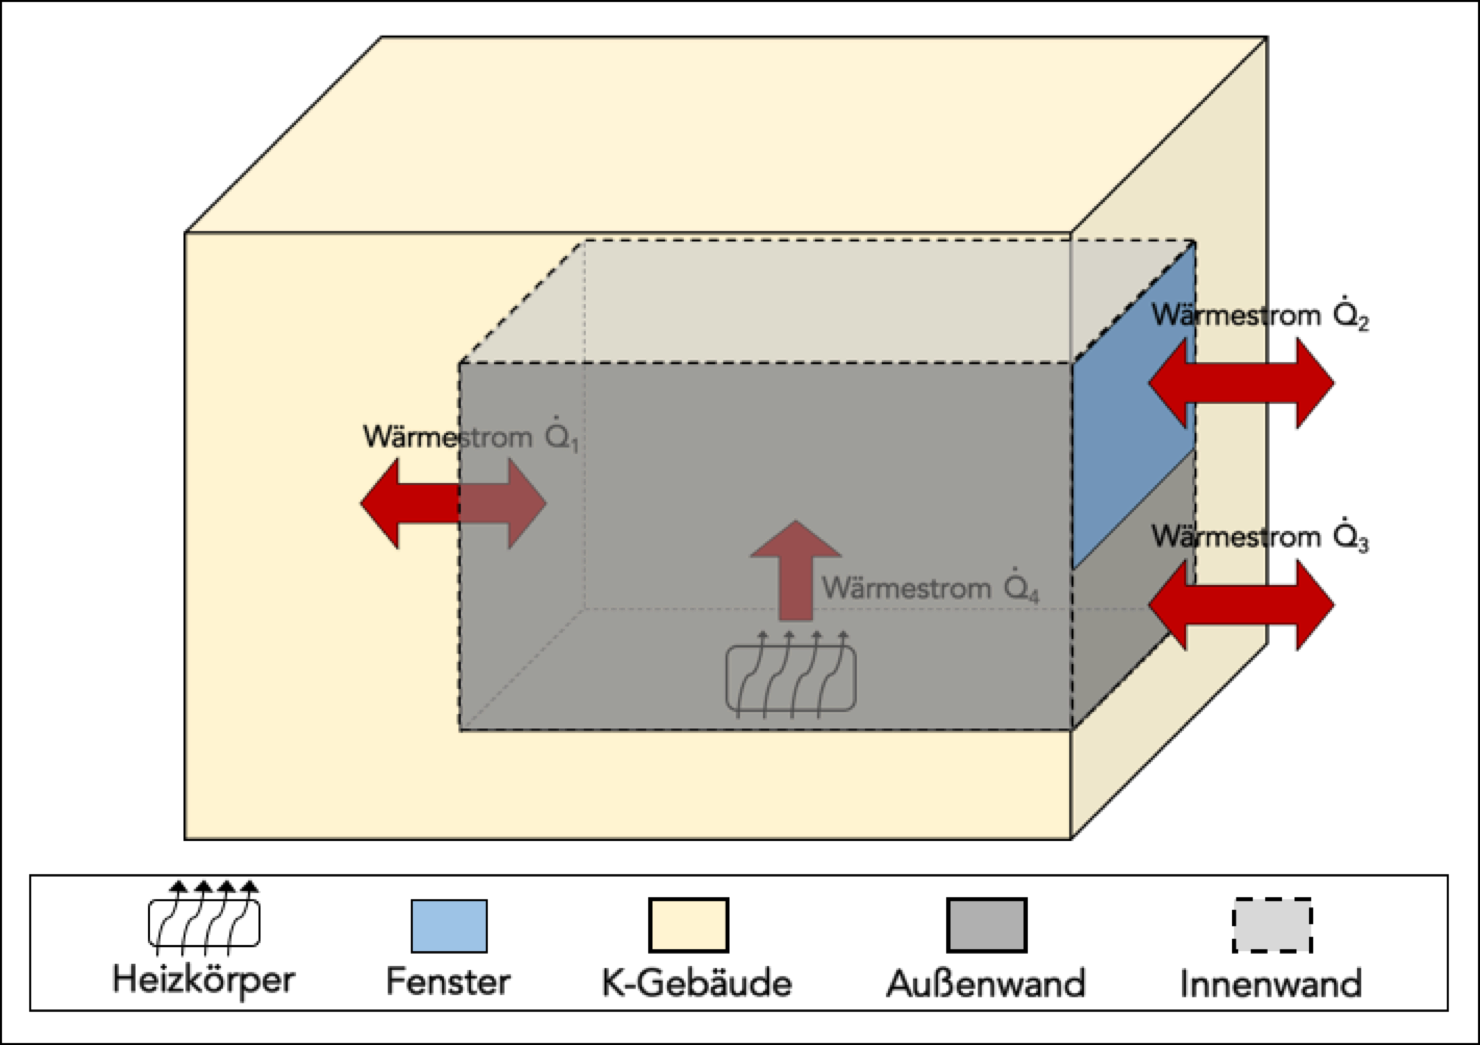
\includegraphics[width=\textwidth]{abbildungen/20160316_raumeins}
\caption{Erweitertes Raummodell}
\label{fig:raumeins}
\end{figure}



\section{Das Heizkörpermodell}

Der Heizkörper im Raum K004b lässt sich nach \cite[S.~824f.]{re14} als Stahlrohrradiator identifizieren. Er besteht aus genormten zwei-säuligen Gliedern jeweils am Sammler oben und unten miteinander verschweißt den Heizkörper bilden.



\begin{table}[H]
\centering
\small
\renewcommand{\arraystretch}{1.3}
\begin{threeparttable}
\begin{tabularx}{1\textwidth}{p{0.5\textwidth}m{0.2\textwidth}m{0.18\textwidth}}
\toprule
\textbf{Modellrelevante Eigenschaften} & \textbf{Wert} & \textbf{Einheit} \\
\cmidrule[0.5pt](r{0.25em}){1-1} 
\cmidrule[0.5pt](l{0.25em}){2-2}
\cmidrule[0.5pt](l{0.25em}){3-3}

Zahl der Glieder & 106\tnote{1)} & $Stück$ \\ 
\ccol Säulen pro Glied & \ccol 2 \tnote{1)} & \ccol $Stück$ \\
Rohrdurchmesser Vertikal & 0,0255\tnote{1)} & $[m}$\\
\ccol Rohrdurchmesser Horizontal & 0,05 \ccol 2 \tnote{1)} & \ccol $m$ \\
Höhe der Glieder & 0,4\tnote{1)} & $[m}$\\
\ccol Länge des Glieds & 0,045 \ccol 2 \tnote{2)} & \ccol $[m]$ \\

Höhe der Glieder & 0,4\tnote{1)} & $[m}$\\
\ccol Länge des Glieds & 0,045 \ccol 2 \tnote{2)} & \ccol $[m]$ \\
Wärmedurchgangskoeffizient Heizkörper & 16\tnote{2)} & $[\frac{W}{m^{2}*K}]$\\

\bottomrule
\end{tabularx}
\begin{tablenotes}[]\footnotesize\singlespacing\setlength\labelsep{0pt}
\item[1)] Wert aus eigener Vermessung des Raumes K004b vom 07.12.2015.
\item[2)] Tabellenwert aus \cite[S.~825]{re14}.
\item[3)] Tabellenwert, geschätzt nach \cite[S.~191ff.]{re14}.
\end{tablenotes}
\end{threeparttable}
\caption{Eigenschaften des Heizkörpermodells}
\label{tab:eigenschaften_heiz}
\end{table}



Bereits bei den Einsatzzielen der Anlage in \ref{sec:anforderungen} war gefordert, den Zusammenhang zwischen der Sonneneinstrahlung und der Raumtemperatur zu untersuchen sowie Störgrößen explizit in Kauf zu nehmen. Daher ist es passend, dass die Fensterfront in Richtung Süden ausgerichtet ist und der Raum K004b als Büro genutzt wird und im nächsten Abschnitt erfolgt eine Anpassung an diese beiden Faktoren.


\section{Modellerweiterung durch Berücksichtigung der Sonneneinstrahlung und Störgrößen}

Der Raum K004b wird regulär als Büro genutzt, weshalb verschiedene Faktoren als Störgrößen in Bezug auf die Raumtemperatur betrachtet werden können. Zum einen wird durch die Menschen und deren Rechner weitere Wärme in den Raum eingebracht und zum Anderen werden die Fenster und die Türen geöffnet und geschlossen. Dabei werden Massenströme zwischen Raum und Außenumgebung sowie K~Gebäude ausgetauscht, welche jedoch zunächst nicht modelliert werden sollen, sondern als Störgröße betrachtet die es durch die Modellprädiktive Regelung zu auszugleichen gilt. Die Wärme von Rechnern und Menschen werden als einfache Wärmequelle im Modell berücksichtigt. 
Zudem trifft auf die südseitigen Fenster Sonnenstrahlung, welche ebenfalls einen Wärmestrom in den Raum einbringt und damit ebenfalls einen Einfluss auf die Raumtemperatur hat. Dieser wird zunächst ebenfalls als eine einfache Wärmequelle aufgefasst.
Damit ergeben sich zwei weitere äußere Steuergrößen, die von der Anlage beziehungsweise dem Modell nicht beeinflusst werden können. Damit erweitert sich das Modell wie folgt:

\begin{lstlisting}[language=Modelica, caption={Erweitertes Gleichungssystem Modell des Raumes unter Berücksichtigung der Sonneneinstrahlung und Störgrößen},label=lst:raumdrei]
equation
   [...]
   /* calculate derivative of the inner energy */
   der(room_u) = environment_qdot + building_qdot + window_qdot + radiator_qdot + sun_qdot + otherfactors_qdot;
\end{lstlisting}

\begin{figure}
\centering
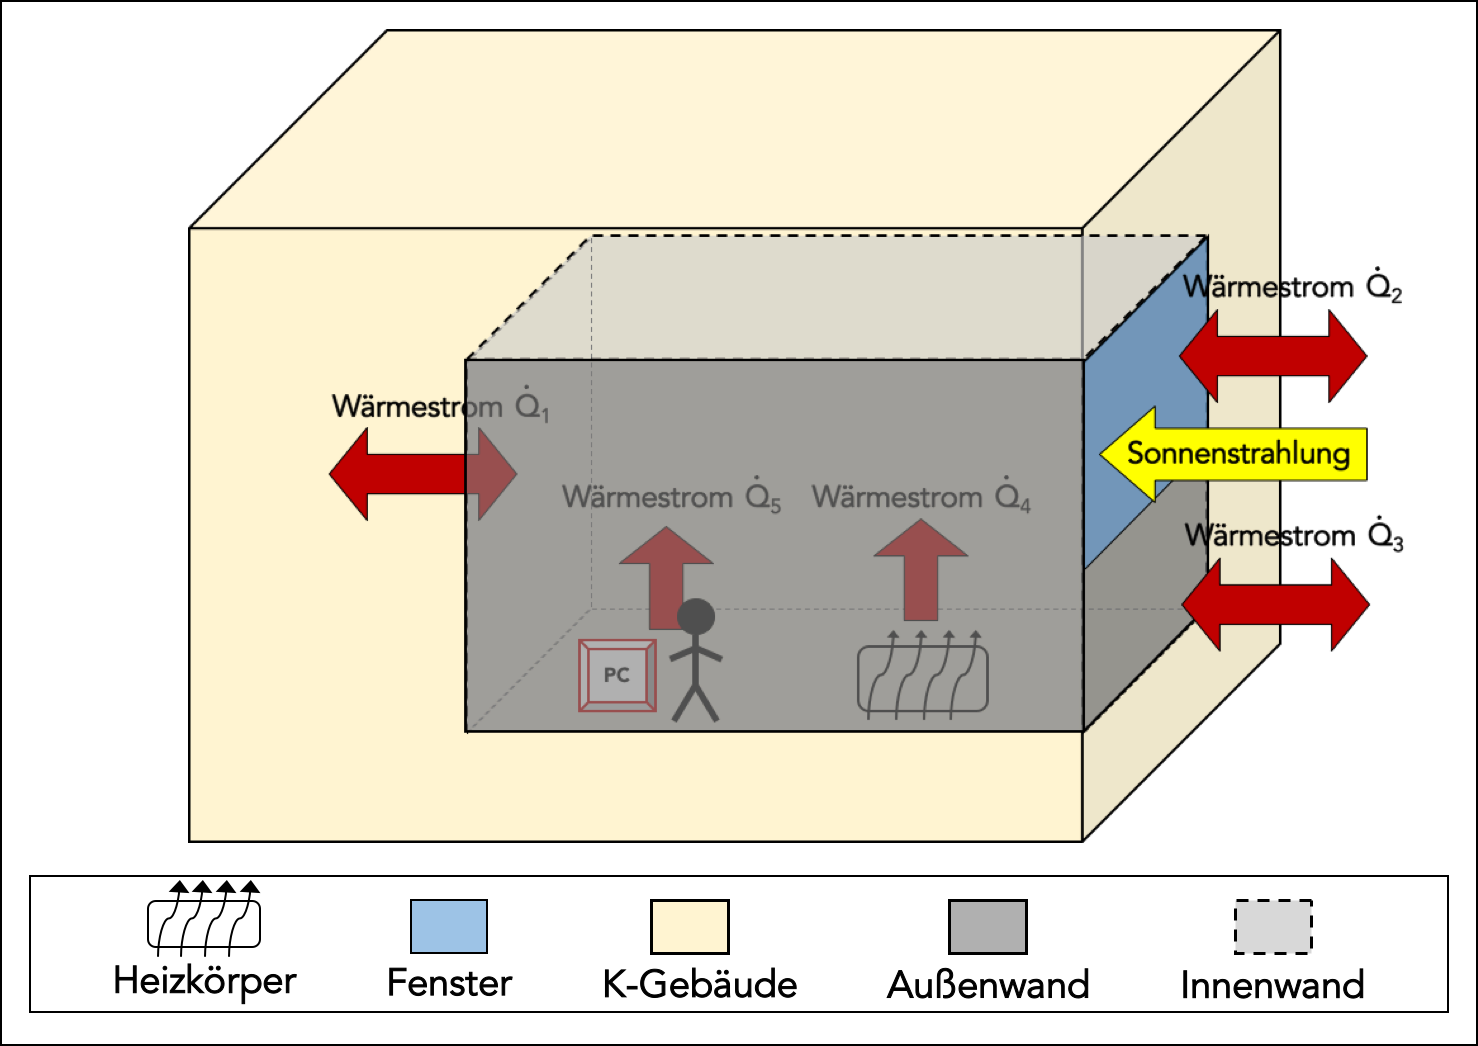
\includegraphics[width=\textwidth]{abbildungen/20160317_raumzwei}
\caption{Erweitertes Raummodell}
\label{fig:raumdrei}
\end{figure}


Damit lassen sich die Zusammenhänge des Modells wie in \ref{fig:raumdrei} visualisieren. Der Einfluss der Sonnenstrahlung wurde bereits in Kapitel \ref{sub:sonne} erläutert und muss nun an die Gegebenheiten des Raumes K004b angepasst werden. Als Messwerte stehen Werte der Globalstrahlung zur Verfügung, welche umgerechnet werden müssen in die effektive Strahlungsintensität an der Fenstersfront.

Da zur Berechnung der effektiven Strahlungsintensität neben der Globalstrahlung auch der Azitmuth und Höhenwinkel der Sonne bekannt sein muss, werden komplexe Berechnungen nötig. Da die Sonnenstrahlung eine Steuergröße darstellt und um die Komplexität des Modells zu schonen, werden die Effektivwerte der Sonnenstrahlung von einem Python Skript berechnet und anschließend dem Modell übergeben. Zudem hat dies den Vorteil, dass im pysolar Package bereits sehr exakte Algorithmen implementiert sind. 
Das Programm ist in Listing \ref{lst:sonne} dargestellt. 
Zur Berechnung des Azimuth- und Sonnenhöhenwinkels wird der Längen- und Breitengrad des K-Gebäudes sowie die Höhe über dem Meerespiegel benötigt. Um die effektive Solarstrahlung zu Bestimmen wird zusätzlich die Ausrichtung der Fensterfläche benötigt. Die Werte sind in Listing \ref{lst:sonne} in Zeile sieben bis zehn zu finden und wurden mit Hilfe von \cite{go15} ermittelt.

\lstinputlisting[language=Python ,caption={Programm zur Umrechnung der Globalstrahlung in die effektive Solarstrahlung an der Fensterfront am Rum K004b}, label=lst:sonne]{listings/radiation_conversion_k004b.py}

Außerdem wird der Startzeitpunkt und der Abstand zwischen den Messpunkten für die gemessenen Daten benötigt, da der Stand der Sonne von der Uhrzeit abhängig ist. Nach dem Einlesen der Messdaten aus der Datei globalstrahlung.csv wird anschließend für jeden einzelnen Messwert und -zeitpunkt der Azimuth- und Sonnenhöhenwinkel berechnet. Darauf basierend wird geprüft, ob die Sonne senkrecht am Himmel steht, noch nicht aufgegangen ist oder die Fläche verschattet ist. Ist dies der Fall trifft keine effektive Strahlung auf das Fenster. Des Weiteren würden sich für niedrige Sonnenstände sehr hohe und unrelistische effektive Strahlungswerte ergeben, weshalb diese für Sonnenstandswinkel kleiner als fünf Grad begrenzt werden.
Ansonsten wird der effektive Strahlungswert nach REFXXXXXgleichung berechnet und in der Datei qdotsun-effective gespeichert. Dieses Programm kann in leicht abgewandelter Form einfach zur Umrechnung einzelner Messwerte genutzt werden, indem das Einlesen und Speichern der umgerechneten Daten durch eine Abfrage eines Messwertes und Übergabe einer Variable mit umgerechnetem Messwert ersetzt wird.

Der effektive Strahlungswert wird allerdings durch den Transmissionsgrad des Fensters weiter abgeschwächt, der durch einen weiteren Paramater/ eine weitere Eigenschaft der $window\_transmission$ beschrieben wird. Der Schätzwert für eine zweischeibige Verglasung des Fensters stammt aus \cite[S.~63]{ha13}. Dadurch erweitert sich das Modell um ein Fenster als Subomponente:

\begin{lstlisting}[language=Modelica, caption={Fenster als Subkomponente des Raummodells},label=lst:raumdrei]
model Window
	Modelica.SIunits.DensityOfHeatFlowRate qdotsun_effective;
	Modelica.SIunits.HeatFlowRate qdot_effective;
	parameter Real window_transmission = 0.5;
	Modelica.SIunits.Area window_surface;
  equation
  	qdot_effective = qdotsun_effective * window_transmission * window_surface;
end Window;
\end{lstlisting}

Das Modell wurde dadurch weiter an die realen Gegebenheiten angepasst 







\section{Validierung des Modells}

\section{Anpassung des Modells mit Parameterschätzung}